\documentclass[letterpaper,11pt]{article}
\usepackage{array}
\usepackage{graphicx}
\usepackage{subcaption}
\usepackage{pdfpages}
\usepackage{changepage}
\usepackage{color}
\usepackage[hyphens,spaces,obeyspaces]{url}
\usepackage[colorlinks=true,urlcolor=blue,citecolor=black]{hyperref}
\usepackage[title]{appendix}

\title{\LARGE BAND\\
    \Large Unleashing Tokenized Economy}
\author{
        Soravis Srinawakoon\\
        \small\href{mailto:soravis@bandprotocol.com}
            {\nolinkurl{soravis@bandprotocol.com}}
    \and
        Sorawit Suriyakarn\\
        \small\href{mailto:swit@bandprotocol.com}
            {\nolinkurl{swit@bandprotocol.com}}
    }
\date{\today\\\small Draft Version 0.1.1}
\begin{document}

\maketitle

\begin{abstract}

Band Protocol is a decentralized, permissionless blockchain protocol to create tokenized marketplace and token-curated community. Band Protocol enables seamless issuance of personalized Community Token through a continuous bonding curve, a smart contract that mints and burned personalized token through a predefined mathematical function based on current circulating supply. Any entities ranging from businesses, brands and celebrities can create a loyal token-curated community with personalized tokens. Personalized Community Token is a utility token representing primary currency, subscription, discount, reward point, or any other use cases within the community as defined by the Community Manager.

Band Protocol standardizes Product Token as a way for community manager to issue products and services. It enables both tokenized real-world products as well as new digital asset creation such as rare digital collectibles and attention token.

Band Protocol enables the creation of subscription business model. Followers can stake their Community Token to a staking contract and receive regular benefits similar to normal subscription or membership. Band Protocol allows Community Manager to define their subscription tier and discount token. Discount token is a tokenized discount voucher used to reward loyal followers and incentivize active participants rather than speculators. The amount of discounts can be customized by Community Manager and in general is proportionate to the amount of total network value. Discount tokens will be an incentive for loyal followers to stake their tokens and promote the growth of the community.

Band Token is the native utility token on the delegated-proof-of-stake Band Chain. Band Token are used to secure the network, provide global liquidity to every Community Token, and act as a governance token for future protocol upgrade.

\end{abstract}

\newpage
{
\hypersetup{linkcolor=black}
\tableofcontents
}
\newpage

\section{Introduction}

\subsection{Tokenized Economy}

A typical market-based economy involves the exchange of goods and services through barter or a medium of exchange. Traditionally, buyers exchange physical coins and banknote with physical products or services offered by sellers. As technology progresses, Internet has enabled digital economy whereby goods and services are being exchanged with digital money. E-commerce experiences exponential growth as people can conveniently conduct transaction with people across the world. Centralized companies start to dominate marketplace platform and payment gateway which are key enablers of the digital economy.

Blockchain and crypto assets are giving rise to yet another revolution in the economy. Bitcoin~\cite{nakamoto}, the first cryptocurrency, becomes the first decentralized currency which enables trustless, censorship-resistant payment. Cryptocurrency such as Bitcoin allows anyone to send transaction to anyone around the world at a fraction of a cost and a fraction of time required for traditional financial institutions to conduct similar transaction. As payment and currency are being tokenized, traditional asset is slower to experience similar tokenization process. Regulation and usability are two key factors that hinder the explosive growth of asset tokenization. Asset tokenization has clear benefits:
\begin{itemize}
\item Global accessibility
\item Liquidity premium
\item Low transaction fee
\item Transparency
\item Security
\end{itemize}

Similar to how physical trade transitions to digital trade by the advancement of the Internet, the next era of commerce is the transition from centralized digital trade to decentralized token trade. Tokenized economy will become prevalent as both real-world assets and payment are being tokenized. Band Protocol enables asset tokenization and creates a standard platform for tokenized economy.
\newpage

\subsection{Token-curated Community}
Typically, economy centers around community with common shared interest. There are multiple layers of community depending on the focus. A country is one big community where everyone shares geographical border, culture, tradition, customs and beliefs. Soccer players and followers together is another community where everyone shares interest in the sport which leads to an economic activity around soccer team and players. This leads to two sides of participant in the community: buyers and sellers. While they share similar interest in the same community, they often have conflicting needs as both sides try to maximize their own utility at the expense of the other side. Soccer team would raise their ticket price as they gain more popularity while their loyal followers have to keep paying more. Conversely, followers will not go out of their way to promote their favorite artist because they have very little economic incentive to do so. Their incentives are not truly aligned.

Crypto asset becomes the answer to which community members can finally have an aligned incentive to grow the community together. A token-curated community is a community centered around a personalized Community Token whose value closely tie to the overall network value of the community. Community Token acts as a shared economic incentive for both buyers and sellers to promote the growth of the community. Band Protocol standardizes the creation of token-curated community and details how personalized Community Token's value can be derived from overall community value through staking and discount mechanism.

%Currently companies, brands and celebrities struggle to engage with their loyal customers and followers. They mostly utilize social media channels such as Facebook, Twitter, and Instagram to cultivate their community. However, it is becoming more difficult to monetize their fan base. Many celebrities try to monetize their followers by advertising products from other companies to their followers, which is not always in the best interest of the community. For example, recent Thai celebrities are facing lawsuit because they advertise non-FDA-approved cosmetics. Influencers accept payment to promote products inorganically which misleads their followers. Similarly, content distributor channel like Youtube and Spotify are taking a big cut from content provider. Newcomers find themselves much more difficult to compete for attention and create network effect, which was originally promised by these platforms.


\subsection{Use Cases}
\begin{itemize}
\item A new musician creates a new community and publishes her first album. She cultivates and rewards early adopters through her Community Token. By having skin-in-the-game token, early adopters rally behind her success and help her grow the community.
\item Bruno Mars issue Bruno Token which can be staked to receive constant discount for all future products, priority queue to purchase concert ticket, and right to access VIP zone during meet and greet session. Bruno Mars also sell rare digital cards which contain non-public photos of the band and digital artwork.
\item Established company creates a community to curate information around a company and reward active participants with community token. Similar to how Barilla encourages followers to post new recipe on Facebook Page, now active participants can receive Barilla Token to purchase Barilla products as an incentive to curate information inside Barilla community.
\end{itemize}

\subsection{BAND Architecture} \label{sec:band-architecture}

BAND architecture consists of three main layers shown in figure~\ref{fig:pyramid}:

\begin{itemize}
\item \textbf{BAND Blockchain Layer} provides backbone blockchain network to support the entire BAND ecosystem. This includes design of cryptographic algorithm for public-private key management, gas allocation, blockchain internal state representation, on-chain price oracle and native BAND Token.
\item \textbf{BAND Protocol Layer} provides standard contracts to facilitate tokenized economy by enabling creation of personalized-token-curated community, tokenized products, token subscription model, discount token, attention curation market, etc.
\item \textbf{Application Layer} is the consumer-facing application that utilize the underlying BAND blockchain and protocol and serve real-world needs. Any developers can create a solution on top of open, permissionless BAND Protocol. Campbase will be the first application built on top of BAND.
\end{itemize}

\begin{figure}[h]
    \centering
    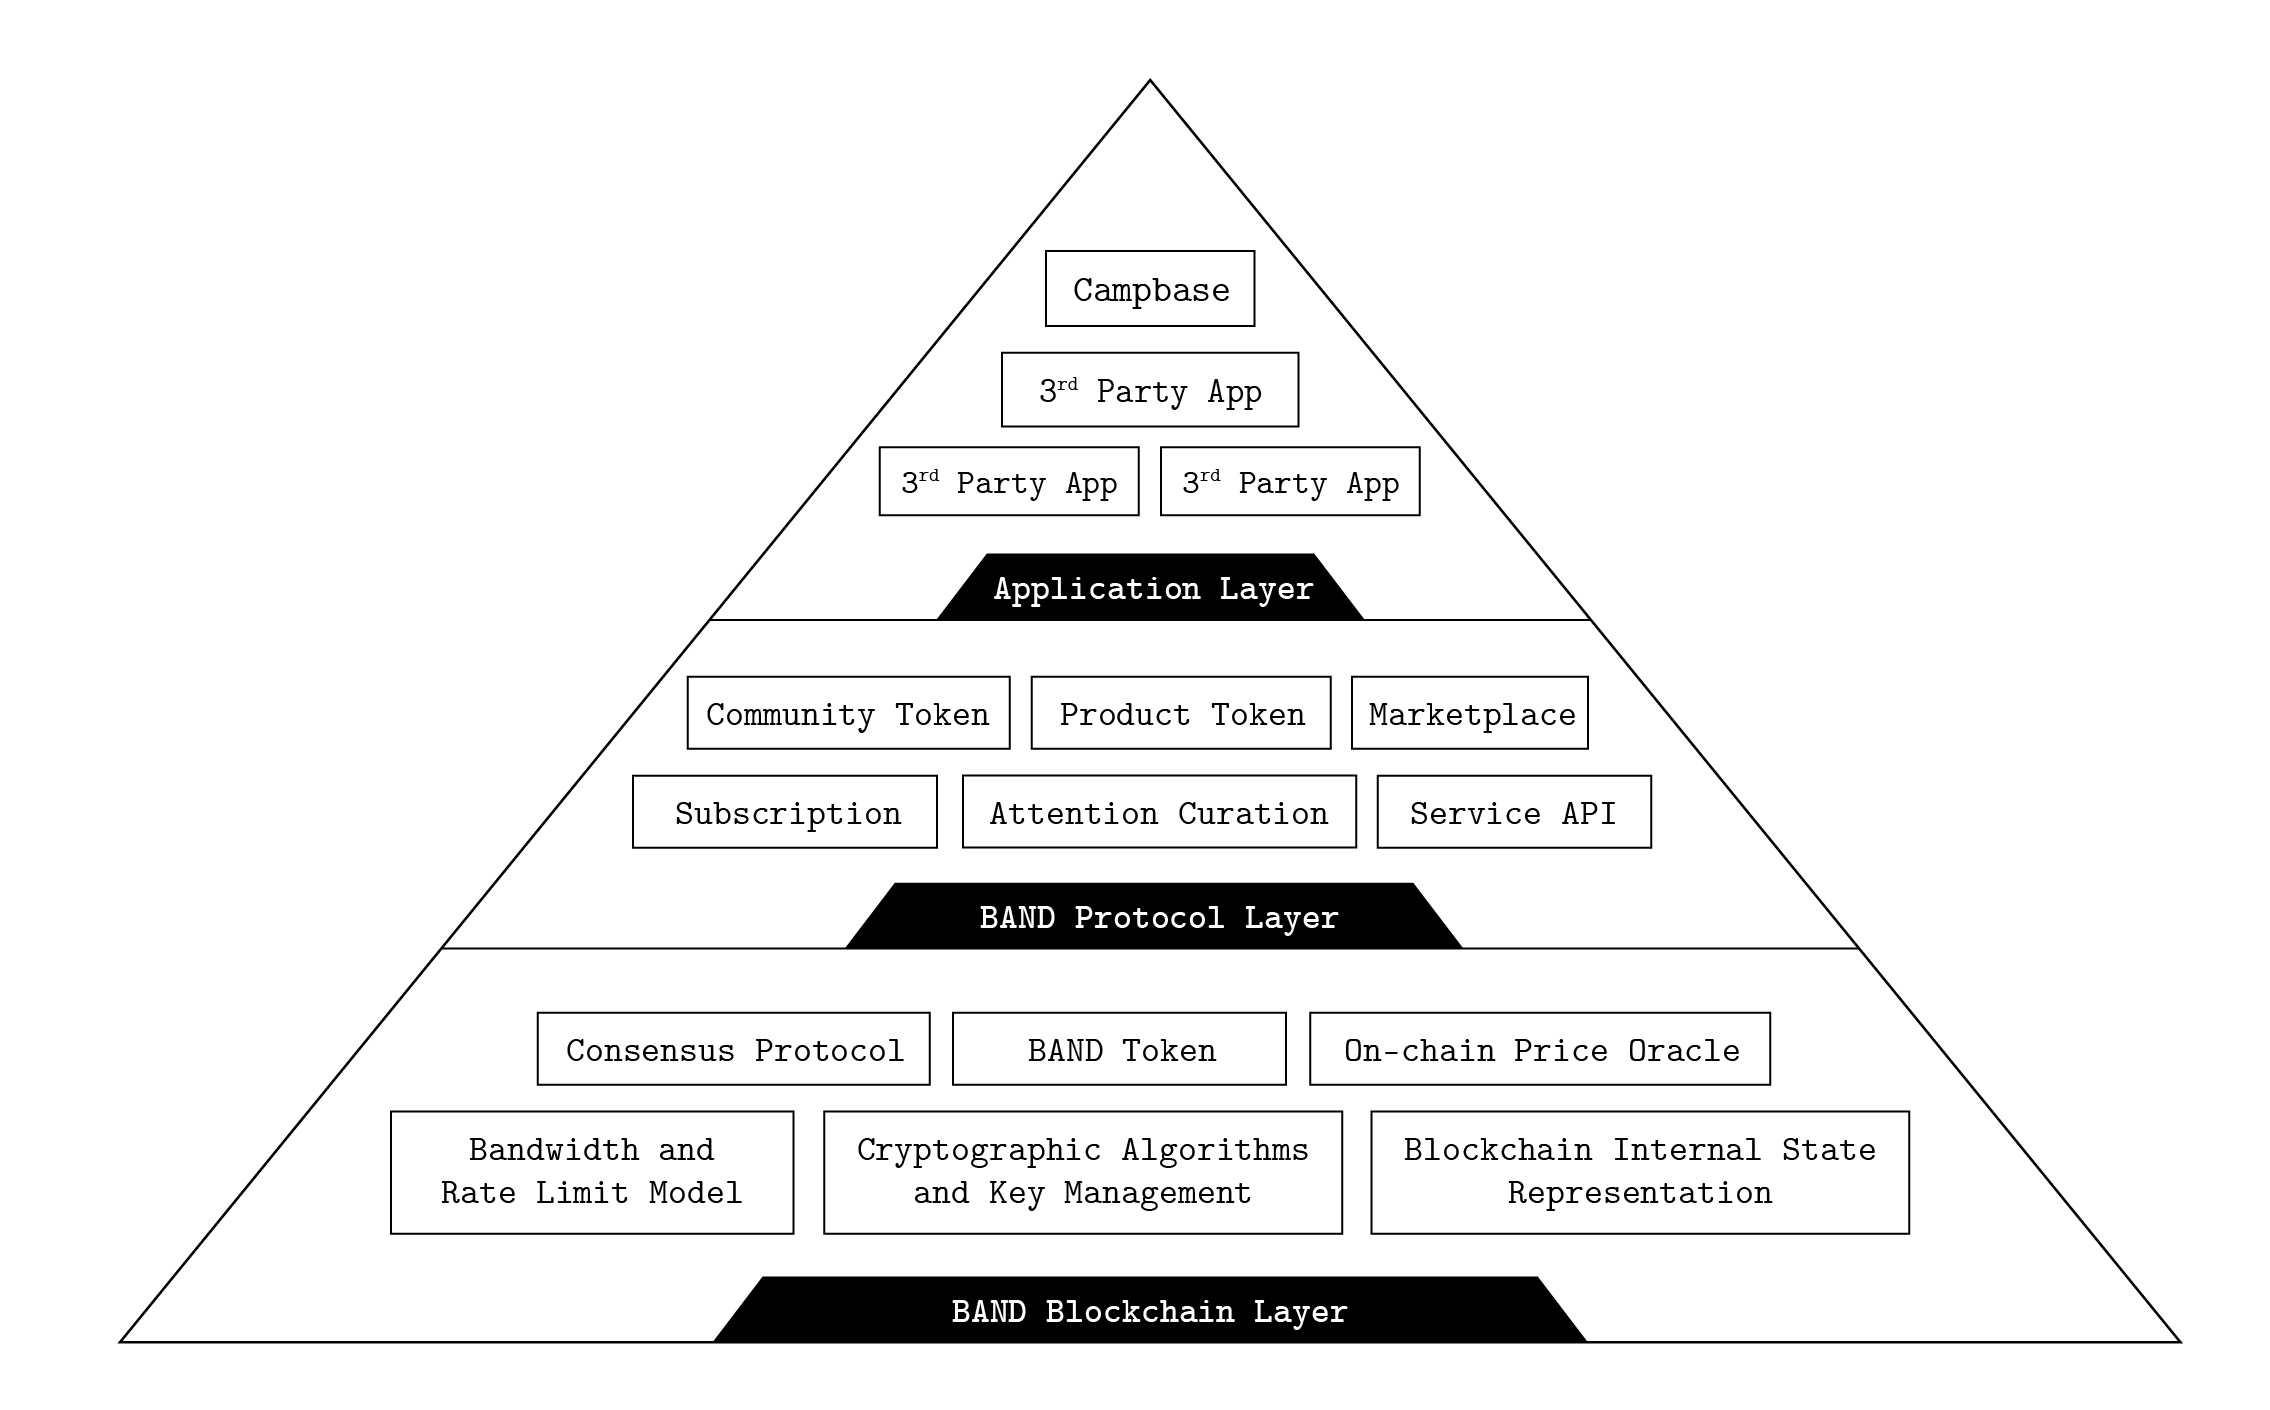
\includegraphics[width=1.05\textwidth]{figures/pyramid}
    \caption{Overview of BAND architecture}
    \label{fig:pyramid}
\end{figure}

\clearpage
\newpage

\section{Blockchain Layer}

\subsection{Delegated Proof-of-Stake Protocol}

\subsubsection{Tendermint}

\subsubsection{Blockchain Parameters}

\subsection{Incentives and Fees}

\subsection{Cryptographic Keys}

\subsection{BAND Protocol State}

\subsubsection{Unspent Transaction Outputs (UTXOs)}

\subsubsection{Static Contracts}

\subsection{On-Chain Price Oracle}

\subsection{BAND Token}

\subsubsection{Staking}

\subsubsection{Bonding}

\subsubsection{Governance and Token-Curated Registries}

\section{BAND Protocol}

\subsection{Community Token}

\subsubsection{Value-Supply Equation}

\subsubsection{Maximum Supply}

\subsubsection{Price Spread}

\subsubsection{Purchase Flow}

\subsection{Product Token}

\subsubsection{Issuance}

\subsubsection{Redemption}

\subsubsection{Beneficiary}

\subsection{Marketplace}

\subsection{Subscription Model}

\subsubsection{Staking Contract}

\subsubsection{Discount Token}

\subsection{Attention Contracts}

\subsection{Service API Contracts}

\section{Client Layer}

\subsection{Campbase}

\subsection{Problem Definition}

\subsection{Solution}

\subsubsection{Story Feed}

\subsubsection{Fan Feed}

\subsubsection{Event}

\subsubsection{Subscription}

\subsubsection{Store}

\subsection{Community Manager}

\subsection{Consumers}

\section{Roadmap}

\bibliographystyle{unsrt}
\bibliography{paper}

\end{document}
